\section{Initialisierung eines lokalen .git}
Git muss in dem Hauptordner eines Projektes initialisiert werden. Das bedeutet, dass alle Projekt-Dateien in Unterordnern zu finden sein müssen (eine Exemplarische Ordnerstruktur ist in \ref{fig:dir_struc} dargestellt). Bei der Initialisierung von Git wird im Hauptordner zusätzlich ein neuer Unterordner  \inline{.git/} angelegt. In diesem Ordner wird Git alle Versionsinformationen und die Historie abspeichern. Durch Löschen des Ordners kann man Git von dem Projekt trennen.
\begin{figure}[!h]
    \dirtree{%
    .1 Git-Basics.
    .2 .git.
    .3 \ldots \hspace{2ex}\begin{minipage}[t]{8cm}In diesem Ordner werden die Informationen über Änderungen abgespeichert\end{minipage}.
    .2 Bilder.
    .3 git\_commit.png.
    .3 Versioncontrol.png.
    .2 main.tex.
    .2 Title.tex.
    .2 initialisierung.tex.
    .2 Einleitung.tex.
    .2 Commit.tex.
    .2 Bibliothek.tex.
    }
    \caption{Exemplarische Ordnerstruktur für ein Projekt mit Git.}
    \label{fig:dir_struc}
\end{figure}

Um in einem Projektordner Git zu initialisieren genügt der Befehl 
\begin{mplisting}
$ git init
\end{mplisting}
Dadurch wird in dem aktuellen Verzeichnis ein \inline{.git} Ordner angelegt.
%
\subsection{Git Config}
Um Änderungen zu protokollieren benötigt Git Informationen über den User. Diese Informationen können System-übergreifend, pro User oder für das jeweilige Projekt hinterlegt werden. Die benötigten Informationen sind Email-Adresse und Benutzername. Definiert werden können die Informationen mithilfe von \inline{git config}. Durch die Angabe einer Option wird definiert ob diese Information für das System (\inline{--system}), den User (\inline{--global}) oder das Projekt (\inline{--local}) abgespeichert werden sollen.
\begin{lstlisting}[breaklines=true]
$ git config --global user.name "Max Mustermann"
$ git config --global user.email "max@mustermann.de"
$ git config --global core.editor vim  # Dieser Editor wird von git genutzt um Eingaben des Users ab zu fragen.
\end{lstlisting}
Nach der Initialisierung kann der Status des Git mit \inline{git status} abgefragt werden.
\begin{mplisting}
$ ls -a
.   Bibliothek.bib  Commit.tex      .git                 main.tex
..  Bilder          Einleitung.tex  initialisierung.tex  Title.tex
$ git status
On branch master

No commits yet

Untracked files:
  (use "git add <file>..." to include in what will be committed)
	Bibliothek.bib
	Bilder/
	Commit.tex
	Einleitung.tex
	Title.tex
	initialisierung.tex
	main.tex

nothing added to commit but untracked files present (use "git add" to track)

\end{mplisting}
Durch diese Initialisierung wurde ein leeres Git-Repository angelegt. Jedoch hat das Repository noch keine Dateien, deren Verlauf protokolliert werden soll. Um Dateien der Versionskontrolle hinzu zu fügen müssen diese zum Repository hinzugefügt werden. Das geschieht über den \inline{git add} Befehl.
\begin{mplisting}
$ git add main.tex
$ git status
On branch master

No commits yet

Changes to be committed:
  (use "git rm --cached <file>..." to unstage)
	new file:   main.tex

Untracked files:
  (use "git add <file>..." to include in what will be committed)
	Bibliothek.bib
	Bilder/
	Commit.tex
	Einleitung.tex
	Title.tex
	initialisierung.tex
\end{mplisting}
Um alle Dateien des Ordners, und der Unterordner dem Repository hinzu zu fügen kann man den Hauptordner hinzufügen.
\begin{mplisting}
$ git add .
$ git status
On branch master

No commits yet

Changes to be committed:
  (use "git rm --cached <file>..." to unstage)
	new file:   Bibliothek.bib
	new file:   Bilder/Versioncontrol.png
	new file:   Bilder/git_commit.png
	new file:   Commit.tex
	new file:   Einleitung.tex
	new file:   Title.tex
	new file:   initialisierung.tex
	new file:   main.tex

\end{mplisting}
Damit wurden alle Dateien der Versionskontrolle hinzugefügt. In Git nennt sich der Zustand, in dem die Dateien sich hier befinden \qq{Staging}. Noch hat Git die Änderungen nicht protokolliert, sondern nur die Dateien markiert um sie bei dem nächsten Commit zu protokollieren. Die vier Stadien, in denen sich eine Datei in Git befinden kann sind in Abb. \ref{fig:lifecycle} dargestellt. Der \inline{git add} Befehl hat die Dateien von \qq{untracked} auf \qq{staged} gesetzt.
\begin{figure}[!h]
    \centering
    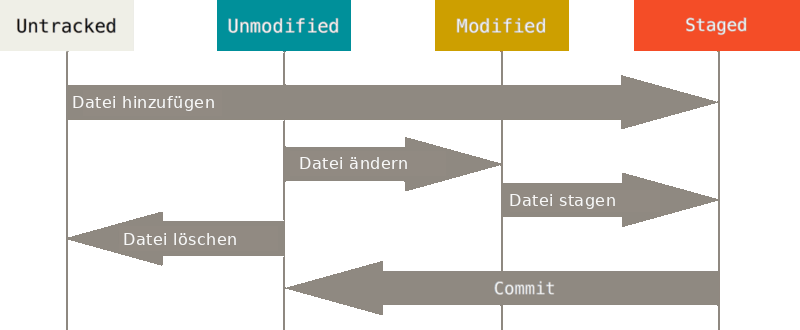
\includegraphics[width=\textwidth]{Bilder/lifecycle_de.png}
    \caption{Die 4 Zustände, in denen eine Datei sich im Git befinden kann. Die Pfeile geben an, wie die Dateien zwischen den Stadien wechseln. Das Bild wurde aus \cite{ProGit} entnommen und leicht verändert.}
    \label{fig:lifecycle}
\end{figure}
